\documentclass[12pt,a4paper]{ctexart}
\usepackage[margin=2.54cm]{geometry}
\usepackage{setspace}\singlespacing
\usepackage{graphicx}\usepackage{booktabs}\usepackage{array}
\usepackage{longtable}\usepackage{tabularx}\usepackage{calc}
\usepackage{caption}\usepackage{url}\usepackage[hidelinks]{hyperref}
\providecommand{\tightlist}{\setlength{\itemsep}{0pt}\setlength{\parskip}{0pt}}
\begin{document}
\begin{titlepage}\centering\vspace*{2cm}
{\Huge\bfseries 第二阶段中期报告\par}\vspace{1.5cm}
{\huge Towards Traceable Stablecoins in Decentralized Finance\par}\vspace{0.6cm}
{\large 面向去中心化金融的稳定币可追溯性：一个基于证据的跨链追踪框架\par}\vfill
{\large \textbf{Student Name:} Tang Tianhao\par}\vspace{0.4cm}
{\large \textbf{Student Number:} 59720490\par}\vspace{1.2cm}
{\large \textbf{Supervisor Name:} Prof LU Zhenliang\par}\vspace{0.4cm}
{\large \textbf{Course:} CS6520 Project\par}\vspace{1.5cm}
\end{titlepage}
\newpage\tableofcontents\thispagestyle{empty}\newpage\setcounter{page}{1}

\hypertarget{ux6458ux8981}{%
\section*{Abstract（摘要）}\addcontentsline{toc}{section}{Abstract（摘要）}\label{ux6458ux8981}}

稳定币已经成为去中心化金融中的核心结算资产。USDT、USDC
等稳定币具有价格稳定、流动性高和跨平台可转移等特点，因此被广泛用于 DeFi
交易、跨境支付、交易所结算和链上套利。然而，同样的特性也使稳定币成为链上洗钱和金融犯罪的重要工具。尤其在跨链桥、流动性池、混币器和中心化交易所共同参与的场景中，资金路径不再局限于单一链上的简单转账图，传统单链追踪方法难以解释资金在何处仍可追踪、何处已经断裂。

本项目研究稳定币交易在 DeFi
环境中的可追溯性。这里的``增强可追溯性''并不是设计新的稳定币协议，也不是声称能够阻止所有洗钱行为，而是构建一个事后追踪框架：只在存在可验证证据时继续追踪稳定币资金路径，在证据不足或协议故意切断输入输出关系时，明确标记为未知协议边界或追踪断点。与依赖金额相似、时间窗口或地址相似度的启发式方法不同，本阶段工作强调
先看证据、再继续追踪，即每条追踪边都需要有明确证据来源。

本报告在第一阶段报告的基础上扩展了方法论、实验分析和项目计划。新增贡献包括：把稳定币资金路径表示为可分析的图；比较不同账本模型对追踪的影响；将跨链桥从原先的“透明/不透明”二分，扩展为按证据强弱分类；实现并运行两个机制不同的真实端到端桥解析案例（Across
Ethereum-to-Arbitrum USDC，liquidity fill；Stargate/LayerZero
Ethereum-to-Arbitrum，message passing）；并系统分析事后追踪在未知桥、不公开一对一关系的桥、混币器、交易所资金池和 DeFi 池化协议中的根本边界。

\hypertarget{introduction}{%
\section{Introduction}\label{introduction}}

\hypertarget{cryptocurrency-money-laundering-at-scale}{%
\subsection{Cryptocurrency Money Laundering at
Scale}\label{cryptocurrency-money-laundering-at-scale}}

区块链技术降低了全球范围内价值转移的门槛。与传统金融系统相比，公链交易具有开放、可验证、无需许可和跨境流动性强等特点。这些特点推动了
DeFi、稳定币、链上交易所和跨链基础设施的发展，但也给 AML/CFT
带来了新的挑战。攻击者可以利用匿名或伪匿名地址、大量中转钱包、DeFi
协议和跨链桥快速移动资金，从而增加追踪成本。

稳定币在这一问题中处于核心位置。相比 ETH、BTC
等波动性较高的资产，稳定币可以在链上长期持有价值而不承受显著价格波动。对于合法用户而言，这使稳定币成为交易、支付和结算工具；对于非法资金而言，这也意味着犯罪收益可以在链上以相对稳定的价值形态快速转移。因此，稳定币的
traceability 已经成为链上合规和 DeFi 安全研究中的重要问题。

稳定币与 BTC、ETH 等普通加密资产存在根本区别。BTC 和 ETH
更接近原生链上资产，其供给、转账和账户状态主要由底层协议规则决定；而主流法币抵押型稳定币，例如
USDT 和 USDC，通常以智能合约 token
的形式发行在公链上，发行方在合约层面保留一个控制面。需要精确说明的是这个控制面\textbf{在什么时候}被使用：发行方并不会干预每一笔普通的点对点转账，其干预集中在几个特定场景------\textbf{发行（issuance，对应储备增发
mint）、赎回（redemption，赎回时 burn）、跨链迁移（cross-chain
migration，通过 burn-and-mint 在链之间转移供应）、风险执行（risk
enforcement，冻结或拉黑特定地址）}。例如，Circle 的跨链传输协议 CCTP
在跨链转移 USDC 时，是在源链 burn、并在发行方背书下于目标链向收款人
mint，而不是一笔普通的 token 转账；Tether 同样针对储备进行
mint/redeem，并曾应执法要求冻结特定地址。这意味着法币型稳定币并不是完全``不可管控''的资产，而是在开放区块链之上嵌入了发行方治理、合规执行和账户控制能力，且这种能力在明确定义的节点上行使，而非持续干预每一笔转账。

这种合约级可管控性构成了稳定币 traceability
的制度和技术基础。一方面，如果发行方能够冻结某些地址，说明稳定币生态已经承认特定地址状态和资金来源具有合规意义；另一方面，如果用户、交易所或监管机构无法解释资金路径，那么冻结、拒收或风险标记就容易变成黑箱操作。因此，对于法币型稳定币而言，追溯能力不是附加功能，而是其可管控逻辑的必要组成部分：只有能够说明资金从哪里来、经过哪些路径、在哪些协议处断裂，链上稳定币的合规治理才具有可解释性。

本项目关注的不是一般意义上的``检测洗钱''，而是更基础的问题：当稳定币在地址、合约、跨链桥、交易所和
DeFi
协议之间流动时，公开数据能够支持我们追踪到哪一步？哪些路径可以由链上日志或协议元数据验证？哪些路径只能作为候选？哪些路径必须停止？

\hypertarget{cross-chain-bridges-and-regulatory-blind-spots}{%
\subsection{Cross-Chain Bridges and Regulatory Blind
Spots}\label{cross-chain-bridges-and-regulatory-blind-spots}}

跨链桥是 DeFi 资金流动的重要基础设施。用户通过桥在
Ethereum、Arbitrum、Optimism、Base、Polygon、BSC、Linea
等链之间迁移资产，从而参与不同生态的交易、借贷、质押和流动性策略。然而，跨链桥也打破了单链交易图的完整性。资金离开源链后，分析者必须判断它是否可以在目标链上继续追踪。

严格来说，一个区块链不能直接向另一个区块链``转账''。Ethereum
上的交易不能直接修改 Linea、Arbitrum 或 Tron
的账本状态。即使两条链上的资产都代表同一种经济标的，例如 USDC 或
USDT，源链上的 token balance 减少也不会自动导致目标链上的 token balance
增加。跨链桥之所以能够实现资产迁移，是因为它在两条链之间建立了一套协议流程：源链上锁定、销毁或托管资产，目标链上释放、铸造或由流动性提供者代付资产。也就是说，跨链桥并不是一笔真正意义上的跨链转账，而是一组被协议连接起来的源链动作和目标链动作。

因此，跨链追溯的核心问题也不是寻找``一笔从链 A 直接转到链 B
的交易''，因为这样的交易在区块链底层并不存在。真正需要追踪的是：源链上的
deposit、lock、burn 或 message
send，是否能够通过公开证据连接到目标链上的 mint、release、fill 或
message execution。这个证据连接可能来自 event log、calldata、message
ID、deposit ID、sequence、VAA 或协议
API。没有这样的连接时，系统只能说明用户与某个桥交互过，不能声称已经知道目标链上的接收方。

现实中的链上洗钱路径往往不是简单的单链多跳转账，而是多跳转账、跨链桥、流动性池、中心化交易所和隐私工具的组合。大型攻击事件，如
Ronin
相关资金流动，说明跨链能力已经成为复杂资金转移路径中的关键组成部分。本报告不声称复现
Ronin
的完整路径，而是将其作为动机：如果一个追踪框架无法处理跨链桥处的路径延续和断裂，它就很难适应真实
DeFi 环境。

公开的链上取证报告已经多次记录攻击者使用 chain hopping、bridges 和
mixers 组合洗钱。Ronin/Axie Infinity 事件中，被盗资金来自 Ronin Bridge
攻击，随后 Lazarus Group 使用 Tornado Cash
等混币服务，并通过跨资产和跨链路径继续转移资金。Harmony Horizon Bridge
事件中，Chainalysis 报告指出相关资金在后续洗钱阶段进入桥协议，并在
Bitcoin 与 Avalanche
等链之间迁移。这些案例说明，跨链桥不仅是被攻击的对象，也可能成为攻击后资金清洗和路径复杂化的一部分。

本报告不会把这些公开案例当作已复现实验结果，而是将其作为研究动机和方法验证方向。当前桥实验选择
Across 与 Stargate/LayerZero
交易，是因为二者暴露了清晰但机制不同的公开证据：Across 提供
\texttt{V3FundsDeposited} 事件、\texttt{depositId} 和
\texttt{/deposit/status} 映射；Stargate/LayerZero 提供 message
metadata、nonce、DVN verification 和 destination
transaction。换言之，公开洗钱案例说明``为什么需要跨链追踪''，Across 与
Stargate case 则说明``当前原型如何在不同桥机制下可复现地完成跨链解析''。

\hypertarget{limitations-of-existing-tools}{%
\subsection{Limitations of Existing
Tools}\label{limitations-of-existing-tools}}

现有工具和研究存在四类限制。

第一，商业区块链分析平台通常具有较广覆盖范围，但其标签来源、跨链解析规则和风险评分方法大多闭源，难以在学术项目中复现和验证。

第二，许多学术方法仍然以单链交易图为主要对象。Bitcoin 的 UTXO 模型和
Ethereum
的账户模型已有大量研究，但跨链桥、流动性池和多链稳定币流动没有被充分整合进一个可解释框架。

第三，部分跨链追踪方法依赖启发式匹配，例如金额相似、时间窗口相近、同一地址在多条
EVM
链上重复出现等。这类方法可以帮助发现候选路径，但其证据强度不足以作为确定性追踪结论。

第四，稳定币追踪需要整合多种证据：ERC-20 Transfer
logs、稳定币发行方冻结列表、OFAC 或其他风险地址、桥合约名单、混币器标签、协议 API 和交易回执。如果不先区分证据强弱，系统就很容易把``识别到桥合约''误写成``已经追到目标链地址''。

因此，本项目采用“先看证据，再继续追踪”的原则。系统只有在存在明确连接证据时才继续追踪；否则，只能把这条路径标记为候选路径、无法确认的协议位置或追踪停止点。

商业工具的做法仍然值得参考。例如 Chainalysis Reactor
的公开产品说明强调在一个调查工作流中追踪 swaps、bridges、DEXs 和
mixers，并将复杂合约活动解释成人类可读的调查步骤。Chainalysis
的洗钱报告也将 chain hopping via cross-chain bridges
作为复杂洗钱策略之一，尤其用于描述 Lazarus Group 等攻击者如何在
mixers、bridges 和多链环境之间切换。本文借鉴这种``follow the money
across
services''的调查视角，但不采用黑箱式风险评分作为核心方法。相反，本项目将其拆解为可复核的证据问题：每次跨链延续都必须说明
源链交易、bridge event、message or deposit
identifier、目标链交易 和证据来源。

\hypertarget{the-passive-taint-problem-for-ordinary-users}{%
\subsection{The Passive Taint Problem for Ordinary
Users}\label{the-passive-taint-problem-for-ordinary-users}}

普通用户可能在完全不知情的情况下收到来自风险地址或高风险路径后继地址的稳定币。交易所和合规系统可能进行多跳回溯，一旦用户收到的资产上游靠近冻结地址、制裁地址、混币器或高风险桥，用户账户就可能被标记。这种现象可以称为被动污染，也就是用户自己没有参与可疑交易，却因为资金来源被牵连。

被动污染说明，可追溯性不仅是执法机构的问题，也是普通用户理解自身资金风险的重要工具。一个可解释的系统应该说明风险来自哪个上游地址、经过几跳、在哪个协议处跨链、证据在哪里、以及追踪在哪里停止。否则，用户只能面对黑箱式风险评分，而无法理解自己为何被标记。

需要说明的是，本阶段把被动污染作为研究动机和可解释性目标，而不是已经完成的量化能力。完整评估还需要计算风险资金占总资金的比例，用来区分``只是轻微接触过风险路径''和``主要资金来源就是风险地址''两种情况。这个比例模型本阶段尚未纳入实验，因此这里只说明问题本身，以及它为什么需要一套先看证据、再解释路径的追踪方法。

\hypertarget{research-objectives}{%
\subsection{Research Objectives}\label{research-objectives}}

本项目的总体目标是增强 DeFi
稳定币交易的可追溯性。本阶段报告将该目标具体化为以下研究问题：

\begin{enumerate}
\def\labelenumi{\arabic{enumi}.}
\tightlist
\item
  如何形式化稳定币资金图，并区分普通地址、风险锚点、桥目标节点、未知协议边界和追踪断点？
\item
  如何根据证据链而不是桥名称，对跨链桥交易进行可追溯性分类？
\item
  当前原型能否在公开链上数据中跑通真实的源链到目标链跨链桥追踪？
\item
  当遇到新桥、未登记桥、不公开一对一关系的桥、混币器、中心化交易所和 DeFi
  池化协议时，事后追踪的边界在哪里？
\end{enumerate}

\hypertarget{scope-stablecoin-traceability-and-current-evm-pilot}{%
\subsection{Scope: Stablecoin Traceability and Current EVM
Pilot}\label{scope-stablecoin-traceability-and-current-evm-pilot}}

本项目题目不是 EVM stablecoins，而是 stablecoin
traceability。因此，理论框架需要讨论不同账本模型和执行模型如何影响可追溯性，包括
UTXO、EVM account
model、Tron、Solana、中心化交易所和链下清算系统。同时，本报告特别关注法币型稳定币，因为
USDT/USDC 等 ERC-20 稳定币具有普通原生加密资产不具备的发行方控制面，例如
mint、burn、freeze 和
blacklist。这些功能使稳定币天然处在``开放转账''和``可管控合规''之间，也使
traceability 成为理解稳定币治理的核心能力。

然而，本阶段实现和实验需要控制范围。端到端跨链桥解析仍聚焦 EVM-like
链，原因是这些链共享 ERC-20 Transfer logs、智能合约事件、\texttt{0x}
地址格式和 Etherscan/Blockscout 类型的数据接口。Tron（TRC-20）和
Solana（program/account 模型、SPL token account）等非 EVM
生态在地址格式、API 和交易结构上都需要单独处理，将 解析模块
扩展到它们留作后续工作。这不是缩小项目题目，而是控制第二阶段实现范围。

\hypertarget{potential-outcome}{%
\subsection{Potential Outcome}\label{potential-outcome}}

本阶段的预期产出包括：一个基于证据的稳定币追踪框架；一个跨链桥证据分类方法；两个机制不同的真实桥解析案例（Across 与
Stargate/LayerZero）；以及对事后追踪根本限制的分析。

\hypertarget{related-work}{%
\section{Related Work}\label{related-work}}

\hypertarget{blockchain-transaction-graphs-and-aml-detection}{%
\subsection{Blockchain Transaction Graphs and AML
Detection}\label{blockchain-transaction-graphs-and-aml-detection}}

区块链 AML
研究最常见的建模方式是将交易历史表示为图：地址、交易、合约或实体作为节点，资金流或交互关系作为边。Weber
et al.~在 Elliptic Dataset 中发布了一个 Bitcoin 交易图基准，包含 203,769
个节点和 234,355 条边，并将 GCN 引入 AML 分类任务；后续 Elliptic2
又进一步提供社区级标注，使研究对象从单个交易扩展到洗钱子图形态。这一系列工作奠定了``链上交易图
+ 风险标签 + 机器学习/图学习''的基本范式。

然而，这类图学习研究主要局限于单链环境。Bitcoin 的 UTXO 模型适合做 coin
lineage 和 input-output taint analysis，但与 DeFi
稳定币合约、跨链桥和流动性池的语义距离较远；Ethereum account model
虽然支持智能合约交互，但合约调用和 ERC-20 Transfer logs
之间并不总是一一对应真实经济控制权变化。例如，一笔稳定币可能经过 DEX
router、bridge pool、vault 或 exchange deposit address，简单地把
\texttt{from} 和 \texttt{to} 地址连成边，容易误解协议中介的作用。

本项目继承交易图方法，但将重点从``分类某个节点是否非法''转向``这条资金路径是否可被证据支持''。换言之，交易图是基础数据结构，而
traceability layer 负责解释边的证据类型、协议语义和断裂位置。这也是
Report 2 相比 Report 1
的主要重心调整：图仍然存在，但图上的每条边必须说明其证据来源。

\hypertarget{cross-chain-transaction-tracing-and-traceability}{%
\subsection{Cross-Chain Transaction Tracing and
Traceability}\label{cross-chain-transaction-tracing-and-traceability}}

跨链交易追踪是与本项目最直接相关的研究方向。Mazorra et al.~在
\emph{Tracing Cross-chain Transactions between EVM-based Blockchains}
中研究 EVM-compatible chains 之间的跨链交易匹配，利用同一私钥在不同 EVM
链上控制相同 \texttt{0x} 地址这一事实，结合时间窗口、金额和 token
类型，将源链 lock/deposit 事件与目标链 mint/release
事件进行匹配。该工作在 Ethereum--Polygon 桥数据上取得较高匹配率，说明
EVM 地址复用确实可以成为跨链匹配信号。

但是，Mazorra
类方法本质上仍包含启发式成分：时间接近、金额相近和地址相同可以提供强候选，但并不总是协议级证明。对于需要合规解释的
stablecoin traceability，候选路径和确定性路径必须区分。若系统无法说明
连接证据 来自 event、calldata、message ID、deposit
ID、sequence、VAA 或官方协议索引器，就不应把匹配结果写成已经追到目标链。

Sun et al.~的 \emph{Track and Trace}
更进一步，将研究对象扩展到多种主流跨链桥，包括 Stargate、Celer
cBridge、Wormhole、Synapse
等。其重要结论是：不同桥的透明度差异很大。Message-passing
或官方桥往往能提供 message ID、sequence、VAA
或目标交易映射；而流动性池、maker/solver 或 pooled bridge
模型可能不暴露一对一 input-output 连接关系。Ren 等人的 tracing survey
也指出，cross-chain tracing 是当前区块链取证中最缺乏统一方法的方向之一。

本项目与这些工作的关系是：我们不否认启发式匹配的发现能力，但将其降级为
candidate generation；真正决定追踪是否继续的是 源链到目标链
连接证据。也就是说，本项目把 cross-chain tracing
从``能否匹配上''改写成``匹配的证据等级是什么''。这直接导向 §4.1 的
evidence type 分类，以及 §5.3 的跨桥 解析模块 状态表。

\hypertarget{multi-hop-risk-scoring-and-tree-based-tracing}{%
\subsection{Multi-Hop Risk Scoring and Tree-Based
Tracing}\label{multi-hop-risk-scoring-and-tree-based-tracing}}

多跳风险评分解决的是另一个核心问题：即使某地址没有直接出现在黑名单上，它是否因为上游或下游路径靠近风险锚点而应被标记？Möser,
Böhme and Breuker 在 Bitcoin 场景中较早系统讨论了 taint
propagation，并区分 poison 和 haircut 两类模型。Poison
模型认为只要资金路径中出现污染输入，后续输出就全部被污染；haircut
模型则按污染资金占总资金的比例传播风险。这一思想为后续 taint analysis 和
proportional exposure 提供了基础。

TaintRank 将污染传播类比为 PageRank，在全局交易图上计算每个地址的 taint
score。它的优势是能给出全网范围的风险分布，缺点是偏离实时单地址查询场景，且仍以单链图为主。Circle
近期的 Transaction Proximity 则从相反方向建模：它计算地址到 regulated
exchange 等合法锚点的距离，用 proximity
解释地址是否处于更可识别、更合规的资金区域。这个方向与本项目互补：Circle
衡量``离合法锚点有多近''，本项目衡量``离风险锚点有多近，以及路径证据是否足够继续''。

这些工作说明，多跳传播不能仅靠固定深度 BFS
粗暴完成。固定深度太浅，会被中转地址绕过；固定深度太深，又会把普通用户卷入远距离污染，产生
被动污染误报。因此，本项目保留 adaptive-depth BFS 和 hop
decay，但把它们服务于稳定币路径追踪：BFS
的目标不是机械地扩大风险邻域，而是构建一棵带证据来源、距离和断点类型的资金路径树；比例暴露则放入最终报告继续实现。

\hypertarget{machine-learning-for-stablecoin-aml}{%
\subsection{Machine Learning for Stablecoin
AML}\label{machine-learning-for-stablecoin-aml}}

StableAML 是当前与稳定币 AML 最接近的机器学习研究之一。Juvinski and Li
使用 16,433 个标注地址和 68 个行为特征训练多个模型，特征覆盖
interaction、transfer、network 和 temporal 四类。其结果显示，CatBoost 等
tree ensemble 在稳定币图上优于复杂
GNN，其中一个重要原因是稳定币交易图较稀疏，GNN
的邻居聚合未必能充分发挥优势，而人工设计的领域特征可以直接表达洗钱行为模式。

这类分类器对候选排序有价值，但高度依赖标签质量和数据规模，且分类器的输出本身并不是对资金路径的解释。因此本项目不把分类模型作为核心贡献，而聚焦
基于证据
traceability：每个结论都由明确的链上或协议证据来源支撑，而非一个学习得到的分数。

\hypertarget{regulatory-frameworks}{%
\subsection{Regulatory Frameworks}\label{regulatory-frameworks}}

FATF 将 virtual assets 和 virtual asset service providers 纳入 AML/CFT
框架，并通过 Travel Rule
要求服务商收集和传递交易相关方信息。稳定币发行方的冻结与黑名单机制、OFAC
sanctions
list、交易所合规筛查共同构成了链上稳定币治理的现实背景。与传统金融不同，DeFi
中大量活动发生在非托管钱包、智能合约和跨链桥之间，监管和风控系统不能只依赖中心化机构内部记录。

EU AI Act 将 AML/CFT 场景中的 AI 系统列为 high-risk AI
systems，这意味着模型不仅要有较高检测性能，还要具有透明性、可解释性和人工监督机制。对本项目而言，这一要求强化了
先看证据
设计的合理性：如果一个地址被标记为风险，系统必须说明风险来自哪条路径、该路径的证据来自哪里、跨链链接是链上自证还是
API 辅助、以及追踪在哪里停止。

因此，监管文献对本项目的启发不是``做一个更高分的黑箱分类器''，而是``构建一个可以解释每一步证据的追踪系统''。这也是为什么本报告将需要协议接口辅助的证据与协议自身提供的证据区分开来，并在 Across
案例中明确区分源链交易回执、协议索引器和目标链交易回执三种证据强度。

\hypertarget{interpretability-and-privacy-preserving-compliance}{%
\subsection{Interpretability and Privacy-Preserving
Compliance}\label{interpretability-and-privacy-preserving-compliance}}

可解释性研究通常关注两个层面：模型为什么给出某个风险分数，以及系统如何把链上行为转换成人类可读的合规解释。Watson,
Richards and Schiff 提出的 explainable blockchain AML 架构将 GNN
detection、GraphLIME attribution 和 LLM explanation
串联起来，试图把黑箱分类结果转成可审查的自然语言报告。Nicholls
等工作也显示，LLM 可以基于交易数据生成可操作的 AML 解释文本。

本项目的解释性重点略有不同：在跨链稳定币 traceability
中，最关键的解释不是``模型为什么预测为高风险''，而是``这条资金边为什么成立''。如果跨链边本身只是启发式猜测，那么再漂亮的自然语言解释也可能是在解释一个未经证明的路径。因此，本项目把解释性前置到
evidence layer：每条边先记录
token-level、协议自身提供、需要协议接口辅助、external-label 或
heuristic signal，再决定是否进入风险评分和自然语言解释。

隐私保护合规提供了另一个长期方向。Buterin et al.~提出的 Privacy Pools /
auditable privacy pools
试图让用户证明资金属于合规集合，或不属于已知非法集合，同时不暴露完整交易历史。Constantinides
and Cartlidge 对 zkMixer 和 proof-of-innocence
类方案的讨论提醒我们：这类协议依赖 blacklist completeness 和 timely
labeling。如果风险地址尚未被标注，隐私池仍可能接收问题资金。因此，当事后追踪在混币器、不公开一对一关系的桥或隐私协议处停止时，协议层合规是重要的后续方向，但并不是本阶段实现目标。

\hypertarget{summary}{%
\subsection{Summary}\label{summary}}

综上，现有研究为本项目提供了四类基础：交易图 AML
提供图建模方法；cross-chain tracing 提供跨链匹配和桥解析背景；taint
propagation 与 Transaction Proximity 提供多跳风险传播思想；StableAML 和
explainable AML
文献提供行为特征与解释性框架。但这些方向仍存在共同缺口：它们往往没有把``跨链边是否成立''作为一等问题来处理。

本项目的定位正是填补这一缺口。它不追求覆盖所有桥，也不把启发式候选写成确定性结论，而是提出一个基于证据的稳定币追踪框架：每条资金边都必须说明证据来源；每个桥交互都必须区分“已经解析到目标链”“需要官方接口辅助”“只能识别为桥合约”“无法确认”和“必须停止追踪”几种情况；当事后追踪遇到混币器、不透明桥、交易所资金池或隐私协议时，系统必须诚实停止。

\hypertarget{system-modeling-and-structure}{%
\section{System Modeling and
Structure}\label{system-modeling-and-structure}}

\hypertarget{architecture-overview}{%
\subsection{Architecture Overview}\label{architecture-overview}}

当前系统可以分为两层。

第一层是资金路径分析。它从稳定币 Transfer logs
中构建资金图，识别普通地址、合约地址、风险锚点、桥合约、混币器、未知协议位置和追踪停止点。

第二层是证据检查。它解释每条边为什么成立，尤其判断跨链桥交易是否可以解析目标链、目标地址或目标交易。Across
与 Stargate 两个案例属于这一层的验证。

\begin{figure}
\centering
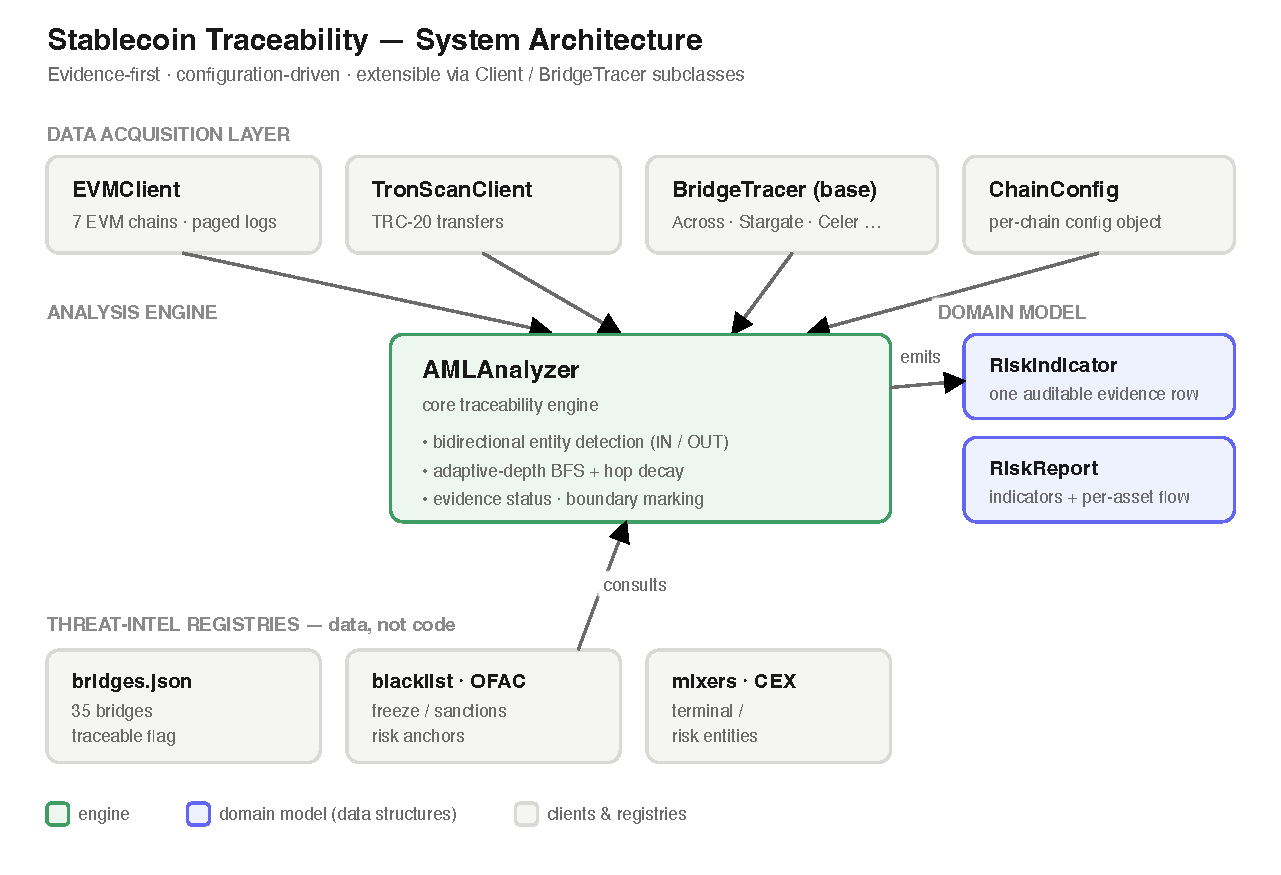
\includegraphics[width=\textwidth]{figures/stablecoin_traceability_architecture_v2.pdf}
\caption{稳定币追踪原型的系统架构。核心 AMLAnalyzer 与链上数据采集模块、桥解析器、风险地址名单和结果数据结构分离。}
\end{figure}

\hypertarget{design-choices-and-justifications}{%
\subsection{Design Choices and
Justifications}\label{design-choices-and-justifications}}

系统的核心设计选择是先看证据、再继续追踪。对于普通稳定币转账，系统依赖 ERC-20 Transfer
logs；对于跨链桥，系统依赖 event logs、calldata、depositId、messageId
或协议 API；对于风险锚点，系统依赖 blacklist、freeze list 或 sanctions
list；对于未知桥和不公开收发关系的协议，系统标记为无法确认的位置或追踪停止点。

这一设计相比启发式方法更保守，但更适合本项目的学术目标。它可以清晰回答：我们知道什么、证据在哪里、哪里还不知道、哪里理论上无法通过公开链上数据恢复。

\hypertarget{methodology-and-algorithms}{%
\section{Methodology and Algorithms}\label{methodology-and-algorithms}}

\hypertarget{traceability-formalization}{%
\subsection{Traceability
Formalization}\label{traceability-formalization}}

稳定币资金图表示为有向图 \texttt{G\ =\ (V,\ E)}。节点 \texttt{V}
包括普通地址、合约地址、风险锚点、桥目标节点、未知协议边界和追踪断点。边
\texttt{E} 表示稳定币转账、跨链桥解析结果或协议辅助映射。

每条边必须包含证据元数据，包括 chain、token、amount、transaction
hash、timestamp、event type、log index 和 resolution
method。根据证据来源，本项目区分以下类型：

\begin{longtable}[]{@{}lll@{}}
\toprule
\begin{minipage}[b]{0.30\columnwidth}\raggedright
Evidence type\strut
\end{minipage} & \begin{minipage}[b]{0.30\columnwidth}\raggedright
Source\strut
\end{minipage} & \begin{minipage}[b]{0.30\columnwidth}\raggedright
Meaning\strut
\end{minipage}\tabularnewline
\midrule
\endhead
\begin{minipage}[t]{0.30\columnwidth}\raggedright
token-level evidence\strut
\end{minipage} & \begin{minipage}[t]{0.30\columnwidth}\raggedright
ERC-20 Transfer log\strut
\end{minipage} & \begin{minipage}[t]{0.30\columnwidth}\raggedright
稳定币在两个地址之间发生转账\strut
\end{minipage}\tabularnewline
\begin{minipage}[t]{0.30\columnwidth}\raggedright
协议自身提供的证据\strut
\end{minipage} & \begin{minipage}[t]{0.30\columnwidth}\raggedright
event log / calldata\strut
\end{minipage} & \begin{minipage}[t]{0.30\columnwidth}\raggedright
协议暴露目标链、目标地址或消息标识\strut
\end{minipage}\tabularnewline
\begin{minipage}[t]{0.30\columnwidth}\raggedright
需要协议接口辅助的证据\strut
\end{minipage} & \begin{minipage}[t]{0.30\columnwidth}\raggedright
official API / explorer\strut
\end{minipage} & \begin{minipage}[t]{0.30\columnwidth}\raggedright
协议索引器提供源链到目标链交易的对应关系\strut
\end{minipage}\tabularnewline
\begin{minipage}[t]{0.30\columnwidth}\raggedright
external-label evidence\strut
\end{minipage} & \begin{minipage}[t]{0.30\columnwidth}\raggedright
blacklist / 名单\strut
\end{minipage} & \begin{minipage}[t]{0.30\columnwidth}\raggedright
地址或合约被外部来源标记\strut
\end{minipage}\tabularnewline
\begin{minipage}[t]{0.30\columnwidth}\raggedright
heuristic signal\strut
\end{minipage} & \begin{minipage}[t]{0.30\columnwidth}\raggedright
time / amount similarity\strut
\end{minipage} & \begin{minipage}[t]{0.30\columnwidth}\raggedright
只能用于候选发现，不作为确定性证据\strut
\end{minipage}\tabularnewline
\bottomrule
\end{longtable}

\hypertarget{accounting-models-and-tracing-constraints}{%
\subsection{Accounting Models and Tracing
Constraints}\label{accounting-models-and-tracing-constraints}}

Traceability
不是所有区块链天然一致的属性，而是取决于账本模型、公开交易数据和协议元数据。

\begin{longtable}[]{@{}lll@{}}
\toprule
\begin{minipage}[b]{0.30\columnwidth}\raggedright
System type\strut
\end{minipage} & \begin{minipage}[b]{0.30\columnwidth}\raggedright
Observable tracing data\strut
\end{minipage} & \begin{minipage}[b]{0.30\columnwidth}\raggedright
Main limitation\strut
\end{minipage}\tabularnewline
\midrule
\endhead
\begin{minipage}[t]{0.30\columnwidth}\raggedright
Bitcoin / UTXO\strut
\end{minipage} & \begin{minipage}[t]{0.30\columnwidth}\raggedright
input-output coin lineage\strut
\end{minipage} & \begin{minipage}[t]{0.30\columnwidth}\raggedright
与 DeFi 稳定币合约生态关系较弱\strut
\end{minipage}\tabularnewline
\begin{minipage}[t]{0.30\columnwidth}\raggedright
EVM fiat-backed stablecoins\strut
\end{minipage} & \begin{minipage}[t]{0.30\columnwidth}\raggedright
ERC-20 logs, mint/burn events, freeze/blacklist state, contract
events\strut
\end{minipage} & \begin{minipage}[t]{0.30\columnwidth}\raggedright
合约中介、router、pool 会改变经济语义\strut
\end{minipage}\tabularnewline
\begin{minipage}[t]{0.30\columnwidth}\raggedright
Native crypto-assets such as ETH\strut
\end{minipage} & \begin{minipage}[t]{0.30\columnwidth}\raggedright
native transfers and transaction traces\strut
\end{minipage} & \begin{minipage}[t]{0.30\columnwidth}\raggedright
缺少稳定币发行方控制面\strut
\end{minipage}\tabularnewline
\begin{minipage}[t]{0.30\columnwidth}\raggedright
Tron / TRC-20\strut
\end{minipage} & \begin{minipage}[t]{0.30\columnwidth}\raggedright
USDT 流通量重要\strut
\end{minipage} & \begin{minipage}[t]{0.30\columnwidth}\raggedright
地址格式和 API 需单独适配\strut
\end{minipage}\tabularnewline
\begin{minipage}[t]{0.30\columnwidth}\raggedright
Solana\strut
\end{minipage} & \begin{minipage}[t]{0.30\columnwidth}\raggedright
token accounts and program invocations\strut
\end{minipage} & \begin{minipage}[t]{0.30\columnwidth}\raggedright
program/account 模型不同\strut
\end{minipage}\tabularnewline
\begin{minipage}[t]{0.30\columnwidth}\raggedright
CEX / custody\strut
\end{minipage} & \begin{minipage}[t]{0.30\columnwidth}\raggedright
deposit and withdrawal addresses\strut
\end{minipage} & \begin{minipage}[t]{0.30\columnwidth}\raggedright
内部账本不可见\strut
\end{minipage}\tabularnewline
\begin{minipage}[t]{0.30\columnwidth}\raggedright
Mixer / privacy protocol\strut
\end{minipage} & \begin{minipage}[t]{0.30\columnwidth}\raggedright
intentionally hidden 连接关系\strut
\end{minipage} & \begin{minipage}[t]{0.30\columnwidth}\raggedright
事后追踪在协议边界断裂\strut
\end{minipage}\tabularnewline
\bottomrule
\end{longtable}

因此，本报告理论上讨论稳定币可追溯性的一般问题，但当前实验聚焦 EVM-like
链。这不是缩小项目题目，而是控制第二阶段实现范围。

在 EVM 法币型稳定币中，traceability 还具有额外意义。由于合约本身支持
mint、burn、freeze 或
blacklist，稳定币已经具备链上治理接口。追踪系统可以为这些治理动作提供解释层：当某个地址被认为存在风险时，系统应能说明它与哪类风险锚点相连、路径证据来自哪些交易和事件、以及在跨链桥或
DeFi 协议处是否仍能继续追踪。换言之，稳定币的可管控性使 traceability
成为必要的中间层，连接链上合约权限和合规解释。

\hypertarget{bridge-名单-and-基于证据-classification}{%
\subsection{Bridge Registry and Evidence-Based
Classification}\label{bridge-名单-and-基于证据-classification}}

跨链桥不是单个合约地址。一次桥接流程可能包含 source
contract、destination contract、message layer、relayer、liquidity pool
和 market
maker。因此，系统不能只根据桥名称判断能否追踪，而要判断具体交易是否暴露
连接证据。

这里需要区分``桥''和``relayer''。桥通常指整个跨链协议或系统，包括源链合约、目标链合约、消息验证、资金池、结算规则和前端/API；relayer 则只是其中一种执行角色，负责把消息提交到目标链，或在目标链先为用户垫付资产。换言之，relayer 不是桥本身，而是桥运行过程中的参与者。对于 Across 这类 liquidity/relayer fill 模型，用户在源链 deposit 之后，目标链收到的资产可能来自 relayer 的先行付款；协议之后再根据 deposit 和 fill 记录与 relayer 结算。因此，追踪时不能简单地把``用户源链付款''和``目标链收款''看成同一笔链间转账，而要找到桥协议公开的 depositId、messageId、fill transaction 或官方状态接口，证明 relayer 的付款确实对应这一次桥接请求。

从原理上看，跨链桥主要解决的是``两个互不共享状态的账本如何表达同一笔资产迁移''。由于链
A 不能直接写入链 B，桥协议通常采用以下几类机制：

\begin{longtable}[]{@{}llll@{}}
\toprule
\begin{minipage}[b]{0.22\columnwidth}\raggedright
Bridge mechanism\strut
\end{minipage} & \begin{minipage}[b]{0.22\columnwidth}\raggedright
Source-chain action\strut
\end{minipage} & \begin{minipage}[b]{0.22\columnwidth}\raggedright
Destination-chain action\strut
\end{minipage} & \begin{minipage}[b]{0.22\columnwidth}\raggedright
Traceability implication\strut
\end{minipage}\tabularnewline
\midrule
\endhead
\begin{minipage}[t]{0.22\columnwidth}\raggedright
lock-and-mint\strut
\end{minipage} & \begin{minipage}[t]{0.22\columnwidth}\raggedright
锁定源链资产\strut
\end{minipage} & \begin{minipage}[t]{0.22\columnwidth}\raggedright
目标链铸造 wrapped asset\strut
\end{minipage} & \begin{minipage}[t]{0.22\columnwidth}\raggedright
需要证明 lock 与 mint 对应\strut
\end{minipage}\tabularnewline
\begin{minipage}[t]{0.22\columnwidth}\raggedright
burn-and-mint\strut
\end{minipage} & \begin{minipage}[t]{0.22\columnwidth}\raggedright
销毁源链 token\strut
\end{minipage} & \begin{minipage}[t]{0.22\columnwidth}\raggedright
目标链铸造 token\strut
\end{minipage} & \begin{minipage}[t]{0.22\columnwidth}\raggedright
需要证明 burn message 与 mint 对应\strut
\end{minipage}\tabularnewline
\begin{minipage}[t]{0.22\columnwidth}\raggedright
lock-and-release\strut
\end{minipage} & \begin{minipage}[t]{0.22\columnwidth}\raggedright
源链锁定或托管\strut
\end{minipage} & \begin{minipage}[t]{0.22\columnwidth}\raggedright
目标链释放已存在流动性\strut
\end{minipage} & \begin{minipage}[t]{0.22\columnwidth}\raggedright
需要证明 release 来自同一 bridge request\strut
\end{minipage}\tabularnewline
\begin{minipage}[t]{0.22\columnwidth}\raggedright
liquidity/relayer fill\strut
\end{minipage} & \begin{minipage}[t]{0.22\columnwidth}\raggedright
用户在源链付款\strut
\end{minipage} & \begin{minipage}[t]{0.22\columnwidth}\raggedright
relayer 或 LP 在目标链垫付\strut
\end{minipage} & \begin{minipage}[t]{0.22\columnwidth}\raggedright
需要 depositId/fillTx 或 API 证明\strut
\end{minipage}\tabularnewline
\begin{minipage}[t]{0.22\columnwidth}\raggedright
message-passing bridge\strut
\end{minipage} & \begin{minipage}[t]{0.22\columnwidth}\raggedright
源链发送 message\strut
\end{minipage} & \begin{minipage}[t]{0.22\columnwidth}\raggedright
目标链执行 message\strut
\end{minipage} & \begin{minipage}[t]{0.22\columnwidth}\raggedright
需要 messageId/nonce/sequence/VAA\strut
\end{minipage}\tabularnewline
\bottomrule
\end{longtable}

这些机制的共同点是：源链和目标链上发生的是两笔或多笔不同交易。桥协议通过消息层、验证者、relayer、liquidity
provider
或官方索引器把它们联系起来。因此，本项目的跨链追踪并不是把两条链上的转账强行看成一条边，而是寻找能够证明两端属于同一桥接动作的
连接证据。

跨链桥也存在天然不足。第一，不同桥没有统一标准接口。Across、LayerZero、Wormhole、Axelar、Celer、Stargate
和 rollup official bridges 暴露的字段和 API
都不同，导致追踪系统必须为不同桥分别写解析代码。第二，桥的安全假设复杂，可能依赖验证者集合、轻客户端、多签、relayer、预言机或流动性提供者。桥一旦被攻击，资产的``跨链表示''和真实抵押资产之间可能出现不一致。第三，流动性桥和
maker/solver
模式下，目标链付款可能由第三方垫付，源链用户与目标链收款之间不一定存在简单的一对一链上转账边。第四，新桥可以随时部署，且不一定立刻有公开
label、文档或 API，这会让系统无法确认它到底把资金送到了哪里。第五，部分桥或聚合器可能故意减少公开信息，使追踪在协议层面变得困难。

这些不足说明，桥的可追溯性不应被理解为``所有桥都能追穿''。更准确的说法是：桥的可追溯性取决于协议是否公开源链到目标链的对应关系。一个桥越清楚地公开
destinationChainId、recipient、messageId、depositId、sequence、VAA，或者直接提供源链交易到目标链交易的对应关系，它就越适合确定性或协议辅助追踪；反之，如果桥只表现为池化资金进出或
maker 代付，而不公开一对一关系，则只能被视为候选路径、无法确认的位置或追踪停止点。

当前原型使用人工整理的桥合约名单来识别已知桥。这个名单不假设覆盖所有桥，因为任何人都可以部署新的类似桥的合约。因此，对于未登记或未验证的新桥，系统不会猜测其目标链路径，而是标记为无法确认。

本项目将桥交互分为五类：

\begin{longtable}[]{@{}lll@{}}
\toprule
\begin{minipage}[b]{0.30\columnwidth}\raggedright
类别\strut
\end{minipage} & \begin{minipage}[b]{0.30\columnwidth}\raggedright
含义\strut
\end{minipage} & \begin{minipage}[b]{0.30\columnwidth}\raggedright
处理方式\strut
\end{minipage}\tabularnewline
\midrule
\endhead
\begin{minipage}[t]{0.30\columnwidth}\raggedright
可直接解析的桥\strut
\end{minipage} & \begin{minipage}[t]{0.30\columnwidth}\raggedright
event/call data 直接暴露目标链和 recipient\strut
\end{minipage} & \begin{minipage}[t]{0.30\columnwidth}\raggedright
继续追踪\strut
\end{minipage}\tabularnewline
\begin{minipage}[t]{0.30\columnwidth}\raggedright
需要官方接口辅助的桥\strut
\end{minipage} & \begin{minipage}[t]{0.30\columnwidth}\raggedright
官方 API 或 explorer 提供源链到目标链交易的对应关系\strut
\end{minipage} & \begin{minipage}[t]{0.30\columnwidth}\raggedright
带 API 证据继续追踪\strut
\end{minipage}\tabularnewline
\begin{minipage}[t]{0.30\columnwidth}\raggedright
只能识别合约的桥\strut
\end{minipage} & \begin{minipage}[t]{0.30\columnwidth}\raggedright
已知桥合约，但当前交易未解析目标地址\strut
\end{minipage} & \begin{minipage}[t]{0.30\columnwidth}\raggedright
标记为候选路径\strut
\end{minipage}\tabularnewline
\begin{minipage}[t]{0.30\columnwidth}\raggedright
无法确认的协议位置\strut
\end{minipage} & \begin{minipage}[t]{0.30\columnwidth}\raggedright
可能是新桥或复杂协议，但没有足够公开信息\strut
\end{minipage} & \begin{minipage}[t]{0.30\columnwidth}\raggedright
停止并标记未知边界\strut
\end{minipage}\tabularnewline
\begin{minipage}[t]{0.30\columnwidth}\raggedright
追踪停止点\strut
\end{minipage} & \begin{minipage}[t]{0.30\columnwidth}\raggedright
不公开一对一关系的桥、混币器、交易所资金池、隐私协议\strut
\end{minipage} & \begin{minipage}[t]{0.30\columnwidth}\raggedright
终止确定性追踪\strut
\end{minipage}\tabularnewline
\bottomrule
\end{longtable}

\hypertarget{cross-chain-resolution-workflow}{%
\subsection{Cross-Chain Resolution
Workflow}\label{cross-chain-resolution-workflow}}

跨链解析的核心目标，是判断源链上的一笔交易能不能和目标链上的一笔执行结果对应起来。常见依据包括：

\begin{itemize}
\tightlist
\item
  \texttt{destinationChainId} 或 \texttt{dstChainId};
\item
  \texttt{recipient}, \texttt{receiver}, \texttt{toAddress};
\item
  \texttt{depositId}, \texttt{transferId}, \texttt{messageId},
  \texttt{nonce}, \texttt{sequence}, \texttt{VAA};
\item
  官方 API 返回的源链交易到目标链交易的对应关系。
\end{itemize}

解析流程如下：

\begin{enumerate}
\def\labelenumi{\arabic{enumi}.}
\tightlist
\item
  识别稳定币交易是否涉及已知桥合约。
\item
  获取源链 transaction receipt。
\item
  解码 event logs 和 calldata。
\item
  提取目标链、目标地址和跨链消息标识。
\item
  如有必要，调用协议 API 或 explorer。
\item
  获取目标链 transaction receipt。
\item
  若对应关系可验证，则加入目标链节点并继续追踪。
\item
  若证据不足，则标记为候选路径、无法确认的位置或追踪停止点。
\end{enumerate}

这个流程可以理解为三步。第一步判断交易对手是不是已知桥合约或桥相关合约。第二步检查这笔具体交易里有没有可验证的跨链证据，例如目标链
ID、recipient、depositId 或 messageId。第三步是在证据足够时切换到目标链继续追踪，在证据不足时停止并标记状态。

因此，桥合约名单本身只回答``这可能是什么协议''，不回答``钱到哪里去了''。真正决定能否继续追踪的，是这笔交易里有没有足够证据。对于 Across 这类 liquidity/relayer fill
模型，源链交易不是直接向目标链转账，而是在 Ethereum 上产生 deposit
event；目标链 Arbitrum 上的资产由 relayer 或流动性系统完成
fill。我们的追踪逻辑通过 \texttt{depositId} 和 Across
\texttt{/deposit/status} API 将源链 USDC deposit 与目标链 fillTx
连接起来。也就是说，系统追踪的是桥协议公开的源链到目标链关系，而不是一笔不存在的链间直接转账。

\hypertarget{adaptive-depth-bfs-and-hop-decay}{%
\subsection{Adaptive-Depth BFS and Hop
Decay}\label{adaptive-depth-bfs-and-hop-decay}}

在单链范围内，系统使用 BFS 扩展稳定币资金图。Hop decay
用于表达风险或污染强度随距离衰减。它不能创造证据，只能对已经存在证据的路径进行距离表达。

对于普通路径，系统使用较小追踪深度；对于靠近风险锚点或桥交互的路径，系统保留更多证据信息。这样可以在覆盖率和误报之间取得平衡。

\hypertarget{preliminary-analysis}{%
\section{Preliminary Analysis}\label{preliminary-analysis}}

本节在项目的核心任务上评估原型：仅用可验证证据，跨越跨链桥重建一条稳定币资金路径。评估围绕两个真实的端到端桥追踪案例展开（§5.1
与
§5.2），二者刻意覆盖\textbf{两种不同的桥机制}，并经\textbf{两个不同的协议索引器}解析。随后给出跨桥对比（§5.3），以及事后追溯的根本极限（§5.4）。

\hypertarget{across-ethereum-to-arbitrum-usdc-bridge-trace}{%
\subsection{Across Ethereum-to-Arbitrum USDC Bridge
Trace}\label{across-ethereum-to-arbitrum-usdc-bridge-trace}}

第一个案例在一笔真实稳定币交易上验证跨链解析工作流：一笔 Across Protocol
V3 的 USDC 从 Ethereum 到 Arbitrum 的转移。

该样本是从公开链上数据中筛选的可复现技术案例，而非洗钱案例。筛选方式是：查询
Ethereum 上 Across V3 SpokePool 合约的 \texttt{V3FundsDeposited}
事件，过滤出 USDC/USDT，并选择一笔事件字段完整、Across status API 返回
\texttt{filled}、且目标链 receipt
可查询的转移。目的是验证解析逻辑能否从源链事件追到目标链 fill
交易，而非对该地址作风险判断。

源链交易为：

\texttt{0x024b2b3cfffddb12ef9b93da592f1ec754c457281b11be4e24324cd26359b3f5}

源链为 Ethereum，桥协议为 Across Protocol V3。系统首先通过 Etherscan V2
API 获取源链 transaction receipt，并定位 \texttt{V3FundsDeposited}
事件。该事件解析出：

\begin{longtable}[]{@{}ll@{}}
\toprule
Field & Value\tabularnewline
\midrule
\endhead
depositId & 1502687\tabularnewline
destination chain & Arbitrum\tabularnewline
destination chain ID & 42161\tabularnewline
depositor &
\texttt{0xcb9055fc2a8f0f27041dc238574100a22df0c15e}\tabularnewline
recipient &
\texttt{0xcb9055fc2a8f0f27041dc238574100a22df0c15e}\tabularnewline
input amount & 40,000.012359 USDC\tabularnewline
output amount & 39,996.803276 USDC on Arbitrum\tabularnewline
\bottomrule
\end{longtable}

随后，系统调用 Across \texttt{/deposit/status} API，通过源链交易哈希和 \texttt{originChainId\ +\ depositId} 查询桥状态。API
返回：

\begin{longtable}[]{@{}ll@{}}
\toprule
\begin{minipage}[b]{0.47\columnwidth}\raggedright
Field\strut
\end{minipage} & \begin{minipage}[b]{0.47\columnwidth}\raggedright
Value\strut
\end{minipage}\tabularnewline
\midrule
\endhead
\begin{minipage}[t]{0.47\columnwidth}\raggedright
status\strut
\end{minipage} & \begin{minipage}[t]{0.47\columnwidth}\raggedright
filled\strut
\end{minipage}\tabularnewline
\begin{minipage}[t]{0.47\columnwidth}\raggedright
destination fill tx\strut
\end{minipage} & \begin{minipage}[t]{0.47\columnwidth}\raggedright
\texttt{0x5f81158cdd5c0ea56c50c6ddbea411e1a08ca031c56fcf057cddc60b0c1cd7ee}\strut
\end{minipage}\tabularnewline
\begin{minipage}[t]{0.47\columnwidth}\raggedright
destination chain ID\strut
\end{minipage} & \begin{minipage}[t]{0.47\columnwidth}\raggedright
42161\strut
\end{minipage}\tabularnewline
\bottomrule
\end{longtable}

最后，系统通过 Etherscan V2 multi-chain API 获取 Arbitrum 上该 fill
transaction 的 receipt，确认目标链交易存在。

该案例属于需要官方接口辅助的可追踪桥。它不是“只能识别合约”，因为系统不仅识别了 Across 合约，还解析出目标链 fill
transaction；它也不是追踪停止点，因为协议公开了可验证的对应关系。整个解析不是基于金额或时间窗口猜测，而是基于源链事件和 Across API。

需要明确指出这条证据链的\textbf{强度并不均匀}。它分为三步：源链交易回执、协议索引器、目标链交易回执。

\begin{enumerate}
\def\labelenumi{\arabic{enumi}.}
\tightlist
\item
  \textbf{源端}：\texttt{V3FundsDeposited} 事件直接从 Ethereum
  交易回执读取并由我们自己解码，其正确性只依赖 Ethereum
  账本的完整性，不依赖任何第三方，由此得到 \texttt{depositId}、目标链 ID
  和 recipient。
\item
  \textbf{协议索引器端}：从 \texttt{depositId} 到目标链 \texttt{fillTx}
  的映射\textbf{无法}仅靠源链推导，因为 fill 是 relayer 之后在 Arbitrum
  上发出的独立交易，源链没有任何字段指向它。我们通过查询 Across
  \texttt{/deposit/status} 索引器获得该映射。因此这一步是
  \emph{需要协议接口辅助}：其正确性依赖 Across
  索引器的诚实与可用性，严格弱于链上自证；若该 API
  停服或返回错误数据，这条链接就无法仅凭公开日志独立重建。
\item
  \textbf{目标端}：我们没有对 API 返回照单全收，而是用返回的
  \texttt{fillTx} 哈希在 Arbitrum
  上拉取真实交易回执，确认该交易确实存在于链上，从而把索引器返回结果重新锚定回可验证的账本数据。
\end{enumerate}

换言之，唯一依赖外部索引器的环节，会被两侧链上交易回执复核。这里要区分两种情况：如果目标地址直接写在源链 calldata 中，证据主要来自链上；如果像 Across 这样需要查询 status API，证据就依赖协议索引器。一个忠实的追溯系统必须记录这种差别，不能把两者当作同等强度的证据。

\hypertarget{stargate-layerzero-message-passing-bridge-trace}{%
\subsection{Stargate / LayerZero Message-Passing Bridge
Trace}\label{stargate-layerzero-message-passing-bridge-trace}}

单个桥案例不足以说明这种方法可以迁移到其他桥。为检验这一点，我们在一个\textbf{机制不同、索引器也不同}的桥上跑了第二个案例：Stargate
经 LayerZero 路由，属于 message-passing 桥（而 Across 是
liquidity/relayer-fill 桥）。Across 的目标端经 Across
\texttt{/deposit/status} API 解析，而 Stargate 的目标端经 LayerZero Scan
解析------后者索引的是跨链\textbf{消息}本身，而非流动性 fill。

源链交易

\begin{verbatim}
0x5955c3c28ee325ae6570793afd7ffb6c4b8416543f4695c739db95b7455485a1
\end{verbatim}

在 Ethereum 上被确认与一个已知 LayerZero endpoint 交互，随后 LayerZero
Scan 返回了该跨链消息及其在目标链上的投递。解析结果见下表。

\begin{longtable}[]{@{}ll@{}}
\toprule
\begin{minipage}[b]{0.47\columnwidth}\raggedright
Field\strut
\end{minipage} & \begin{minipage}[b]{0.47\columnwidth}\raggedright
Value\strut
\end{minipage}\tabularnewline
\midrule
\endhead
\begin{minipage}[t]{0.47\columnwidth}\raggedright
bridge family\strut
\end{minipage} & \begin{minipage}[t]{0.47\columnwidth}\raggedright
Stargate（message-passing via LayerZero）\strut
\end{minipage}\tabularnewline
\begin{minipage}[t]{0.47\columnwidth}\raggedright
source chain\strut
\end{minipage} & \begin{minipage}[t]{0.47\columnwidth}\raggedright
Ethereum（srcEid 30101）\strut
\end{minipage}\tabularnewline
\begin{minipage}[t]{0.47\columnwidth}\raggedright
destination chain\strut
\end{minipage} & \begin{minipage}[t]{0.47\columnwidth}\raggedright
Arbitrum（dstEid 30110）\strut
\end{minipage}\tabularnewline
\begin{minipage}[t]{0.47\columnwidth}\raggedright
message GUID\strut
\end{minipage} & \begin{minipage}[t]{0.47\columnwidth}\raggedright
\texttt{0xcc519912\ldots{}450c14}\strut
\end{minipage}\tabularnewline
\begin{minipage}[t]{0.47\columnwidth}\raggedright
nonce\strut
\end{minipage} & \begin{minipage}[t]{0.47\columnwidth}\raggedright
82123\strut
\end{minipage}\tabularnewline
\begin{minipage}[t]{0.47\columnwidth}\raggedright
LayerZero status\strut
\end{minipage} & \begin{minipage}[t]{0.47\columnwidth}\raggedright
DELIVERED（executor transaction confirmed）\strut
\end{minipage}\tabularnewline
\begin{minipage}[t]{0.47\columnwidth}\raggedright
DVN verification\strut
\end{minipage} & \begin{minipage}[t]{0.47\columnwidth}\raggedright
3 个 required DVN：LayerZero Labs、Nethermind、Canary（均
SUCCEEDED）\strut
\end{minipage}\tabularnewline
\begin{minipage}[t]{0.47\columnwidth}\raggedright
destination tx\strut
\end{minipage} & \begin{minipage}[t]{0.47\columnwidth}\raggedright
\texttt{0xc4740664\ldots{}91cfd16}（Arbitrum 上 receipt 已观测）\strut
\end{minipage}\tabularnewline
\bottomrule
\end{longtable}

该案例与 Across
一样，也按``源链交易回执、协议索引器、目标链交易回执''的顺序完成验证，但有两点差异强化了泛化性主张。其一，中间步由不同索引器承担（LayerZero
Scan，而非 Across
API），说明该追踪流程不绑定某一个协议的工具。其二，message-passing
模型暴露更丰富的验证元数据：LayerZero 消息携带 GUID、nonce
和一组去中心化验证者网络（DVN）背书------此处是三个 required
DVN（LayerZero Labs、Nethermind、Canary）全部
\texttt{SUCCEEDED}。因此被索引的中间环节不是单一不透明的 API
断言，而是带有独立验证者状态的消息记录，其信任基础强于单一 relayer-fill
查询。和之前一样，目标链交易回执在 Arbitrum
上被拉取以重新锚定该声称。Across（liquidity fill）和 Stargate（message
passing）两个案例都经不同索引器端到端解析后，说明该追踪流程至少适用于两种不同的桥机制。

\hypertarget{cross-bridge-cases-and-current-status}{%
\subsection{不同跨链桥的解析方式和当前完成情况}\label{cross-bridge-cases-and-current-status}}

上面两个案例覆盖了两种桥机制；本小节把它们放到更广的图景中，并如实说明当前代码在其他桥上能走到哪一步。下表不是在夸大覆盖范围，而是在区分四种状态：有的桥已经完成了从源链到目标链的真实解析；有的只有解析代码初稿，还没有跑通完整案例；有的只能识别为桥合约；有的协议本来就不公开一对一的收发关系，因此只能把追踪停在这里。

\begin{longtable}[]{@{}llll@{}}
\toprule
\begin{minipage}[b]{0.22\columnwidth}\raggedright
桥或桥类型\strut
\end{minipage} & \begin{minipage}[b]{0.22\columnwidth}\raggedright
基本方式\strut
\end{minipage} & \begin{minipage}[b]{0.22\columnwidth}\raggedright
如何连接源链和目标链\strut
\end{minipage} & \begin{minipage}[b]{0.22\columnwidth}\raggedright
当前完成情况\strut
\end{minipage}\tabularnewline
\midrule
\endhead
\begin{minipage}[t]{0.22\columnwidth}\raggedright
Across V3\strut
\end{minipage} & \begin{minipage}[t]{0.22\columnwidth}\raggedright
liquidity/relayer fill\strut
\end{minipage} & \begin{minipage}[t]{0.22\columnwidth}\raggedright
\texttt{V3FundsDeposited} 事件 + \texttt{depositId} +
\texttt{/deposit/status} API → fill tx\strut
\end{minipage} & \begin{minipage}[t]{0.22\columnwidth}\raggedright
已完成源链到目标链解析\strut
\end{minipage}\tabularnewline
\begin{minipage}[t]{0.22\columnwidth}\raggedright
Stargate\strut
\end{minipage} & \begin{minipage}[t]{0.22\columnwidth}\raggedright
message-passing (LayerZero)\strut
\end{minipage} & \begin{minipage}[t]{0.22\columnwidth}\raggedright
已知 endpoint + LayerZero Scan API（message GUID、nonce、DVN set）→ 目标链交易\strut
\end{minipage} & \begin{minipage}[t]{0.22\columnwidth}\raggedright
已完成源链到目标链解析\strut
\end{minipage}\tabularnewline
\begin{minipage}[t]{0.22\columnwidth}\raggedright
Celer cBridge\strut
\end{minipage} & \begin{minipage}[t]{0.22\columnwidth}\raggedright
lock-and-release\strut
\end{minipage} & \begin{minipage}[t]{0.22\columnwidth}\raggedright
\texttt{Send} 事件（\texttt{transferId}, \texttt{receiver},
\texttt{dstChainId}）+ cBridge API\strut
\end{minipage} & \begin{minipage}[t]{0.22\columnwidth}\raggedright
有解析初稿但未跑通\strut
\end{minipage}\tabularnewline
\begin{minipage}[t]{0.22\columnwidth}\raggedright
Rollup official\strut
\end{minipage} & \begin{minipage}[t]{0.22\columnwidth}\raggedright
lock-and-mint (canonical)\strut
\end{minipage} & \begin{minipage}[t]{0.22\columnwidth}\raggedright
deposit 事件；源地址在 L2 上保留（同一 \texttt{0x}）\strut
\end{minipage} & \begin{minipage}[t]{0.22\columnwidth}\raggedright
只能识别合约\strut
\end{minipage}\tabularnewline
\begin{minipage}[t]{0.22\columnwidth}\raggedright
Orbiter / Synapse\strut
\end{minipage} & \begin{minipage}[t]{0.22\columnwidth}\raggedright
pooled / maker fill\strut
\end{minipage} & \begin{minipage}[t]{0.22\columnwidth}\raggedright
无公开一对一源链到目标链关系\strut
\end{minipage} & \begin{minipage}[t]{0.22\columnwidth}\raggedright
协议本身不公开\strut
\end{minipage}\tabularnewline
\bottomrule
\end{longtable}

由此有两点。其一，解析方法逐桥不同：Across 和 Stargate 的最后一步都需要查询官方或协议相关的索引服务，分别是 Across status API 和 LayerZero Scan；而 rollup 官方桥在一些情况下可以直接依靠链上事件和同一个用户地址继续分析。其二，表里的“当前完成情况”只写已经做到的事。Across 和 Stargate 有真实交易和保存下来的解析结果；Celer 只有代码初稿，尚不能作为实验结果；Rollup official 目前只是能识别合约；Orbiter 和 Synapse 这类资金池或做市模式，本身就不公开一对一关系，所以不能硬说已经追到目标链地址。

\hypertarget{fundamental-limits-of-post-hoc-tracing}{%
\subsection{Fundamental Limits of Post-hoc
Tracing}\label{fundamental-limits-of-post-hoc-tracing}}

公开区块链并不意味着资金路径总是可追踪。事后追踪能不能继续，取决于协议是否公开足够的信息。

本项目识别出以下边界：

\begin{enumerate}
\def\labelenumi{\arabic{enumi}.}
\tightlist
\item
  未知桥或未登记合约：新桥可能确实在执行跨链功能，但没有公开标签、文档或稳定的事件格式；
\item
  不公开一对一关系的桥：maker、solver 或 pooled liquidity 模式可能只显示资金池进出，而不公开源链用户和目标链收款人的直接对应关系；
\item
  混币器或隐私协议：协议目的就是切断输入和输出之间的关系；
\item
  中心化交易所或托管资金池：链上只显示充值和提现，内部账本不可见；
\item
  DeFi 协议里的资金混合：AMM、vault、lending pool 和 aggregator
  可能在正常业务逻辑中混合资金。
\end{enumerate}

因此，本系统不会通过启发式猜测伪造确定性路径，而是在这些位置明确停止，或者只保留为候选线索。

这一点也解释了本项目与商业链上分析平台的区别。Chainalysis
等商业工具通常将链上数据、服务标签、OSINT、专有聚类和调查工作流结合起来，以支持执法和合规调查。公开资料显示，Chainalysis
Reactor 强调跨多条链、资产、bridges、DEXs 和 mixers
的一体化追踪能力；其洗钱报告也将 cross-chain bridges 和 mixers
视为复杂洗钱路径的重要组成部分。本项目不具备商业平台的私有标签和实体聚类能力，也不试图复刻其闭源评分。相反，本项目选择一个较窄但可复核的目标：在公开链上数据和公开协议元数据范围内，明确哪些跨链路径有证据、哪些只是候选、哪些必须断裂。这样的定位更适合作为学术原型，并能避免把不可验证的黑箱判断误写为确定性追踪。

\hypertarget{milestones-and-overall-schedule}{%
\section{Milestones and Overall
Schedule}\label{milestones-and-overall-schedule}}

本节说明这次报告相比第一次报告具体推进了什么。第一次报告主要是在打基础：先说明为什么稳定币会成为链上洗钱和合规问题里的重点资产，再讨论普通用户为什么可能在不知情的情况下收到有风险来源的资金，同时整理了跨链桥、混币器、交易所和监管要求这些背景。代码方面，第一次报告已经有了早期的地址分析程序，能够读取部分稳定币转账记录，也开始尝试用转账次数、收发关系、金额分布等地址特征描述风险行为。换句话说，第一次报告解决的是“这个问题为什么重要”和“可以从哪些链上数据开始做”。

这次报告的变化，是把题目从宽泛的“反洗钱检测”收紧到“稳定币资金能不能被解释清楚地追下去”。这不是简单换一个说法，而是研究重点的改变。单纯给一个地址打风险分，并不能告诉用户或分析人员风险从哪里来；如果资金跨过一座桥，也不能说明这笔钱在另一条链上到了哪里。因此，这次报告把重点放在路径解释上：每继续追一步，都要说明依据是什么；如果依据不够，就明确停下，而不是用金额相似或时间接近去硬连。

第一阶段留下的数据和代码并没有被推翻，而是被重新组织。早期收集的稳定币转账记录、黑名单地址、桥合约名单、混币器和交易所标签，在这次报告里被用来判断一条资金路径是否有公开证据支持。原来只把桥粗略分成“透明”和“不透明”，现在改成看具体交易能不能解析：有的桥会在链上事件里直接写出目标链和收款地址；有的桥需要查询官方接口才能找到目标链交易；有的只能确认用户进了某个桥，但不知道目标链收款方；还有的桥、混币器或交易所资金池本来就不公开一对一关系。这样写的目的，是让系统少做猜测，多说明“为什么能追”和“为什么不能追”。

实验上，这次报告最重要的结果是两个真实跨链桥案例。Across 案例从 Ethereum 上的一笔 USDC 跨链交易开始，先读出 Across 合约事件里的 \texttt{depositId}、目标链和收款人，再通过 Across 的状态接口找到 Arbitrum 上对应的 fill 交易，最后检查 Arbitrum 上这笔交易确实存在。Stargate/LayerZero 案例则不是流动性垫付模式，而是跨链消息模式：系统通过 LayerZero Scan 找到消息编号、nonce、验证状态和目标链交易。两个案例放在一起说明，我们不是只对一个桥做了特例，而是在两种不同的跨链方式上都跑通了“源链交易到目标链交易”的解析过程。

这次报告还加入了 Solana 和 Tron，但说法比较克制。Solana 的 CCTP 例子不是完整跨链追踪，而是说明同一个稳定币跨链协议到了非 EVM 链上，证据不再是 ERC-20 的 Transfer 事件，而要看 program 调用、账户列表和 SPL 代币余额变化。Tron 的 USDT 例子也不是完整跨链追踪，而是说明 TRC-20 转账可以读出发送方、接收方和金额，但如果要继续解析跨链桥或交易所内部换链，还需要单独处理 Tron 的地址格式和数据接口。因此，这两条链在本阶段只是证明“数据能读、证据形式不同”，不是声称已经完整支持所有非 EVM 链。

总体来说，第二阶段已经把项目从“做一个泛泛的 AML 风险工具”推进到“解释稳定币资金路径能追到哪里”的方向。第一次报告给了背景、数据和早期代码；这次报告把它们变成了更清楚的实验路线：先定义什么证据可以支持一条路径，再区分不同桥能不能解析，然后用 Across 和 Stargate 两个真实案例证明方法可以运行，最后说明哪些地方必须停止。后续如果继续做，重点不应该是盲目增加很多链和很多桥，而是选择少数有代表性的桥，把每个实验的输入交易、解析步骤和输出结果写清楚，让读者能看明白报告里的结论是怎么来的。

\hypertarget{references}{%
\section{References}\label{references}}

正式英文报告将使用 BibTeX 管理参考文献。外部图表和数据将按 guideline
要求引用来源。由本项目实验生成的表格和图，也会说明对应的实验记录和数据来源。

本报告当前应补充的参考来源包括：Chainalysis Reactor product
page（用于说明商业工具如何描述跨链、DEX、mixer 调查工作流）；Chainalysis
2024 Crypto Money Laundering Report（用于说明 chain hopping via
cross-chain bridges 和 mixers
在现实洗钱中的作用）；以及相关跨链追踪论文，例如 Track and Trace /
ABCTRACER，用于支撑 bridge 连接证据 和 cross-chain transaction
identification 的学术背景。

\end{document}
